% Sablon pentru realizarea lucrarii de licenta, conform cu recomandarile
% din ghidul de redactare:
% - https://fmi.unibuc.ro/finalizare-studii/

% Multumiri lui Gabriel Majeri, acest sablon a fost creat pe baza
% codului sursa a lucrarii sale de licenta. 
% Codul sursa: https://github.com/GabrielMajeri/bachelors-thesis
% Website: https://www.gabrielmajeri.ro/
%
% Acest sablon este licentiat sub Creative Commons Attribution 4.0 International License.
% modificat 8 noiembrie 2024

\documentclass[12pt, a4paper]{article}

% Suport pentru diacritice și alte simboluri
\usepackage{fontspec}
% Font Times New Roman
\setmainfont{Times New Roman}

% Suport pentru mai multe limbi
\usepackage{polyglossia}

% Setează limba textului la română
\setdefaultlanguage{romanian}
% Am nevoie de engleză pentru rezumat
\setotherlanguages{english}

% Indentează și primul paragraf al fiecărei noi secțiuni
\SetLanguageKeys{romanian}{indentfirst=true}

% Suport pentru diferite stiluri de ghilimele
\usepackage{csquotes}

\DeclareQuoteStyle{romanian}
  {\quotedblbase}
  {\textquotedblright}
  {\guillemotleft}
  {\guillemotright}

% Utilizează biblatex pentru referințe bibliografice
\usepackage[
    maxbibnames=50,
    sorting=none
]{biblatex}

\addbibresource{bibliography.bib}

% Setează spațiere inter-linie (doublespacing din LaTeX este echivalentul setarii 1.5 in Microsoft Word)
\usepackage{setspace}
\doublespacing

% Modificarea geometriei paginii (cu margini de 2,5 cm) 
\usepackage[margin=2.5cm]{geometry}

% Include funcțiile de grafică
\usepackage{graphicx}
% Încarcă imaginile din directorul `images`
\graphicspath{{./images/}}

% Listări de cod
\usepackage{listings}

% Linkuri interactive în PDF
\usepackage[
    colorlinks,
    linkcolor={black},
    menucolor={black},
    citecolor={black},
    urlcolor={blue}
]{hyperref}

% Comenzi matematice
\usepackage{amsmath}
\usepackage{mathtools}

% Simboluri matematice codificate Unicode
\usepackage[warnings-off={mathtools-colon,mathtools-overbracket}]{unicode-math}

\usepackage{array}
\usepackage{float}
\usepackage{algorithm}
\usepackage{algpseudocode}
% Formule matematice
\newcommand{\bigO}[1]{\symcal{O}\left(#1\right)}
\DeclarePairedDelimiter\abs{\lvert}{\rvert}

% Suport pentru rezumat în două limbi
% Bazat pe https://tex.stackexchange.com/a/70818
\newenvironment{abstractpage}
  {\clearpage\pagestyle{empty}}
  {\clearpage}
\renewenvironment{abstract}[1]
  {\bigskip\selectlanguage{#1}%
   \begin{center}\bfseries\abstractname\end{center}}
  {\par\bigskip}

% Suport pentru anexe
\usepackage{appendix}
\usepackage{tocloft}

% Stiluri diferite de headere și footere
\usepackage{fancyhdr}

\usepackage{chngcntr}
\counterwithin{figure}{section}
\counterwithin{table}{section}

% Metadate
\title{DNS Tunneling Securizat: Implementarea unui protocol de transport fiabil și rezilient la rate limiting}
\author{Stîngă Alexandru-Ionuț}

% Generează variabilele cu @
\makeatletter

\begin{document}

% Front matter
\cleardoublepage
\let\ps@plain

% Pagina de titlu
\include{0-title}
\restoregeometry
\newgeometry{
    margin=2.5cm
}

\fancypagestyle{main}{
  \fancyhf{}
  \renewcommand\headrulewidth{0pt}
  \fancyhead[C]{}
  \fancyfoot[C]{\thepage}
}

\addtocounter{page}{1}

% Rezumatul
\begin{abstractpage}

\begin{abstract}{romanian}
Concomitent cu progresul tehnologic, perimetrele de securitate ale sistemelor informatice și ale rețelelor au devenit mult mai stricte. Cu toate acestea, sistemul DNS încă rămâne un important vector de atac, susceptibil la comunicațiile ascunse.
În această lucrare sunt prezentate structura, implementarea și evaluarea unui protocol securizat, bidirecțional, încadrat în tipologia Command-and-Control și exfiltrare de date. Acesta este construit exclusiv pe infrastructura DNS, având ca obiectiv principal conturarea unui nivel de transport fiabil, capabil să reziste mecanismelor de protecție automată a rețelelor, în special limitării ratei de transfer.
Scopul este atins prin integrarea unui mecanism propriu de control al fluxului de trafic, de tip Stop-and-Wait ARQ. De asemenea, confidențialitatea și integritatea datelor sunt asigurate prin utilizarea algoritmilor ECDHE pentru stabilirea cheii de criptare, AES-GCM pentru criptarea și decriptarea autentificată a mesajelor, și HMAC cu un secret pre-partajat pentru prevenția atacurilor Man-in-the-Middle.
Testele de performanță au demonstrat reziliența protocolului prin menținerea integrității datelor transferate în condiții de limitare a ratei impuse de ISP și de resolverii DNS. Așadar, lucrarea evidențiază amenințarea persistentă a canalelor ascunse și dovedește abilitatea primitivelor criptografice moderne, împreună cu un control riguros al fluxului, de a asigura transmiterea viabilă de date chiar și sub constrângerile dure impuse de rețelele contemporane.
\end{abstract}

\begin{abstract}{english}
Alongside technological progress, the security perimeters of information systems and networks are hardening. Still, the Domain Name System remains an important attack vector, exploitable by covert communication.
This thesis presents the structure, implementation and evaluation of a secure, bidirectional Command-and-Control and data exfiltration protocol. It is built exclusively over stateless DNS, its main objective being the engineering of a reliable transport layer capable of withstanding modern automated network defenses, specifically rate limiting. 
This is achieved by integrating a custom Stop-and-Wait Automatic Repeat Request mechanism. Furthermore, the confidentiality and integrity of the payload are enforced using Ephemeral Elliptic Curve Diffie-Hellman for the establishment of the cryptographic key, AES-GCM for authenticated message encryption and decryption, and HMAC based on a master key for preventing Man-in-the-Middle attacks.
The benchmarks have shown the resilience of the protocol by maintaining the integrity of the transferred data against the rate limiting of the ISP and DNS resolvers. Ultimately, the thesis emphasises the persistent threat brought by covert communication and proves the ability of modern cryptographic primitives, combined with strict flow control, to secure a viable data transfer channel even under contemporary network restrictions.
\end{abstract}

\end{abstractpage}

\tableofcontents
\thispagestyle{empty}

% Main matter
\cleardoublepage
\pagestyle{main}
\let\ps@plain\ps@main

\section{Introducere}

\subsection{Contextul actual}
În contextul curent al securității cibernetice, zonele de protecție ale rețelelor private au devenit foarte restrictive. Folosirea pe scară extinsă a aplicațiilor avansate de tip Firewall, precum NGFW, și a sistemelor de detectare și protecție împotriva infiltrărilor neautorizate, asemenea IDS sau IPS, a dus la blocarea automată a majorității porturilor și protocoalelor de comunicație ce nu sunt esențiale. Cu toate acestea, există o excepție arhitecturală esențială, anume Domain Name System (DNS).

Întrucât rezoluția numelor de domeniu reprezintă o componentă importantă pentru funcționarea internetului, traficul pe portul 53, adesea folosit de protocoalele UDP și TCP, este rar filtrat sau blocat în întregime. Din acest motiv, infrastructura DNS devine un vector de atac propice stabilirii canalelor ascunse. Astfel, prin încapsularea datelor arbitrare în interiorul cererilor și răspunsurilor DNS legitime, tehnică cunoscută sub numele de DNS Tunneling, comunicarea reușește să ocolească politicile stricte de securitate impuse de sistemele informatice. Deși inițial utilizată pentru evitarea portalurilor captive din cadrul rețelelor publice, tehnica a fost răspândită în cadrul exploatărilor de tip Command-and-Control și pentru exfiltrarea silențioasă a datelor din medii izolate. 

\subsection{Obiectivele lucrării}
Principalul scop al acestei lucrări de licență, încadrată în subdomeniul securității cibernetice și al rețelelor de calculatoare, este planificarea structurii, implementarea și evaluarea unui protocol de transport personalizat. Acesta garantează o comunicare bidirecțională fiabilă și sigură doar prin utilizarea QNAME-urilor și a înregistrărilor de tip TXT din DNS.

Spre deosebire de aplicațiile tradiționale ce au la bază mecanisme de tip \textit{Sliding Window}, lucrarea prezintă o arhitectură adaptată să reziste la mecanismele moderne de apărare, mai ales la limitarea ratei de transfer dictată de furnizorii de servicii internet și resolverii publici. Obiectivele concrete includ:

\begin{itemize}
    \item \textbf{Dezvoltarea unui nivel de transport fiabil:} Proiectarea unui sistem de control al fluxului de tip Stop-and-Wait Automatic Repeat Request, care să gestioneze pierderile de pachete (de exemplu, \textit{ACK loss}) și să funcționeze pe post de formator implicit de trafic pentru evitarea declanșării protecțiilor anti-DDoS.
    \item \textbf{Securizarea canalului de comunicație:} Implementarea unui sistem criptografic solid ce respectă triada CIA: Confidențialitate, Integritate și Disponibilitate. Se utilizează schimbul de chei Ephemeral Elliptic Curve Diffie-Hellman pentru obținerea cheii de criptare simetrică, AES-GCM pentru criptarea autentificată a datelor și HMAC bazat pe un secret pre-partajat pentru prevenirea atacurilor de tip Man-in-the-Middle.
    \item \textbf{Implementarea funcționalităților de Command-and-Control:} Crearea unei arhitecturi de tip client-server multi-thread capabilă să susțină încărcarea și descărcarea fișierelor, dar și execuția într-un mediu securizat a comenzilor shell la distanță. 
\end{itemize}

\subsection{Structura tezei}
Structura lucrării este:

\textbf{Capitolul 2: Preliminarii} prezintă baza teoretică pe care protocolul este construit, extrapolând funcționarea canalelor ascunse prin DNS, constrângerile inerente acestora, dar și primitivele criptografice moderne utilizate. De asemenea, acest capitol include o analiză a soluțiilor actuale, evidențiindu-se necesitatea abordării propuse. 

\textbf{Capitolul 3: Arhitectura și implementarea sistemului} detaliază principalul grad de inovație realizat în lucrare. Sunt reliefate designul modular al aplicației, matematica fragmentării datelor pentru trimiterea pachetelor, mașina de stări a procesului de \textit{handshake}, cât și logica mecanismului de Stop-and-Wait ARQ pentru tratarea erorilor ce pot apărea pe rețea.  

\textbf{Capitolul 4: Evaluarea Performanțelor și Rezultate} descrie metoda de testare și analizează performanța protocolului într-un context real de rețea. Se interpretează rezultatele referitoare la asimetria lățimii de bandă și latenței, demonstrându-se totodată reziliența arhitecturii la limitările ratei de transfer. De asemenea, se realizează o analiză a pachetelor folosind \textit{Wireshark}.

\textbf{Capitolul 5: Concluzii} rezumă rezultatele obținute, validează îndeplinirea obiectivelor propuse și discută posibilele direcții de dezvoltare și optimizarea ulterioară a protocolului.
\section{Preliminarii}

Acest capitol stabilește fundamentul teoretic necesar pentru a înțelege arhitectura protocolului personalizat. În continuare, se explică funcționarea sistemului DNS ca mediu de transport și se analizează setul de primitive criptografice alese pentru securizarea canalului de comunicare. De asemenea, tot în această secțiune este prezentat stadiul curent al cercetării în domeniul canalelor ascunse, împreună cu limitările inerente ale soluțiilor existente.

\subsection{Concepte fundamentale ale rețelei}
Analiza modului de operare al sistemului DNS este esențială. Prin natura sa, DNS este un protocol \textit{stateless} bazat pe UDP (portul 53), conceput exclusiv pentru rezoluția numelor de domeniu. Serverul tratează fiecare cerere independent, clientul fiind obligat să trimită constant toate datele de stare.

\subsubsection{Mecanismul de tunelare prin DNS}
Deși rolul DNS-ului este corespondența nume-IP, neglijarea securității acestui protocol permite exploatări precum \textit{DNS Tunneling}. Arhitectura cere un domeniu controlat, un client compromis și un server de tunelare configurat ca \textit{name server autoritativ} pentru acel domeniu~\cite{farnham_dns_tunneling}.

Deoarece informațiile exfiltrate nu pot fi transmise în text clar, ele sunt codificate. Metodele comune includ \textit{Base32} pentru atașarea datelor ca subdomeniu în eticheta QNAME și \textit{Base64} pentru secțiunea RDATA~\cite{farnham_dns_tunneling}. 

Standardul pentru o tunelare robustă folosește înregistrări \textbf{TXT}, care permit șiruri arbitrare de până la 255 de octeți. Răspunsurile DNS pot conține multiple șiruri TXT, permițând un transfer \textit{downstream} superior celui \textit{upstream}. Mai mult, extensia EDNS depășește limita tradițională de 512 octeți a pachetelor UDP. Totuși, protocolul impune restricții stricte QNAME-urilor: o etichetă (porțiunea delimitată de puncte) nu poate depăși 63 de octeți, iar lungimea totală a numelui de domeniu este limitată la 255 de octeți~\cite{farnham_dns_tunneling}.

\subsubsection{Limitările și protecțiile rețelelor}
Rețelele sunt prudente cu protocoalele UDP deoarece facilitează atacurile de tip \textit{Denial-of-Service} (DoS). DNS este o țintă perfectă din trei motive principale~\cite{isc_rrl}:

\begin{itemize}
    \item \textbf{Lipsa verificării sursei:} Software-ul (ex. BIND) nu poate valida sursa pachetului, permițând falsificarea adresei pentru a viza o victimă.
    \item \textbf{Politici ISP permisive:} Lipsa filtrării pachetelor falsificate la ieșirea din rețea facilitează atacurile de reflectare (\textit{Reflection Attacks}).
    \item \textbf{Asimetria traficului:} O interogare \textbf{ANY} de 36 de octeți poate genera răspunsuri de peste 3500 de octeți. Această amplificare de 100 de ori este fundația atacurilor \textit{DNS Amplification}.
\end{itemize}

Deoarece filtrarea răspunsurilor legitime este dificilă, operatorii utilizează \textit{Response Rate Limiting} (RRL). Acest mecanism detectează răspunsurile similare frecvente folosind o schemă \textit{token bucket}. Fiecare combinație client-răspuns consumă un credit; la epuizarea acestuia, pachetele sunt aruncate (\textit{packet loss}), limitând rata de transfer~\cite{isc_rrl}.

Suplimentar, echipamentele \textit{Next-Generation Firewalls} (NGFW) utilizează analize statistice. Deoarece \textit{payload}-ul este codificat în QNAME, domeniile rezultate prezintă o entropie informațională ridicată față de cele standard. Tunelele maximizează transferul (etichete de 63 de octeți, domenii de 255 de octeți) și generează nume cu o densitate nefirească de cifre. Din acest motiv, tunelurile tradiționale sunt foarte susceptibile la detecția automată~\cite{farnham_dns_tunneling}.

\subsection{Primitive criptografice}
Securitatea oferită de protocoalele criptografice tradiționale (precum TLS) este dificil de implementat peste DNS din cauza constrângerilor de dimensiune a pachetelor și a naturii \textit{stateless} specifice UDP. Așadar, lucrarea utilizează o suită de primitive moderne, selectate pentru eficiența spațială și robustețea matematică în context pre-cuantic.

\subsubsection[Schimbul de chei (ECDHE)]{Schimbul de chei: Ephemeral Elliptic Curve Diffie-Hellman (ECDHE)}
\textit{Diffie-Hellman} (DH) stabilește un secret comun pe un canal nesecurizat. Algoritmul implică un grup $\mathbf{G}$ de ordin $p$ (număr prim mare) cu un generator $g$. Părțile generează $a, b \in \mathbb{Z}_{p}^{x}$ și schimbă cheile publice $h_A= g^{a}$ și $h_B= g^{b}$, calculând secretul comun $K_A=h_B^{a}=h_A^{b}=K_B$. Securitatea se bazează pe dificultatea calculării logaritmului discret. Criptografia pe curbe eliptice (ECC) aplică aceste principii pe structura algebrică a curbelor eliptice, oferind un nivel de securitate echivalent dar utilizând chei semnificativ mai mici (\textit{Elliptic Curve Diffie-Hellman} - ECDH).

Modul efemer (ECDHE) utilizează cheile generate pentru o singură sesiune. Odată stabilit secretul comun, calculele anterioare sunt eliminate, garantând \textit{Perfect Forward Secrecy} (PFS); compromiterea ulterioară a unei chei nu permite decriptarea traficului trecut. Conform standardelor NIST~\cite{nist_sp800_56Ar3}, secretul comun nu trebuie utilizat direct ca o cheie de criptare simetrică sau ca vector de inițializare, ci trebuie procesat printr-o schemă de derivare, precum \textit{HKDF}~\cite{rfc5869}, care execută doi pași:

\begin{itemize}
    \setlength{\itemsep}{0pt}
    \setlength{\parskip}{0pt}
    \item $\text{HKDF-Extract}(salt, \text{IKM}) \rightarrow \text{PRK}$
    \item $\text{HKDF-Expand}(\text{PRK}, info, L) \rightarrow \text{OKM}$
    \begin{itemize}
        \setlength{\itemsep}{0pt}
        \setlength{\parskip}{0pt}
        \item \textbf{salt -} valoare aleatoare opțională (implicit, un șir de zerouri de lungime \textit{HashLen}).
        \item \textbf{IKM -} materialul inițial (\textit{Input Keying Material} - secretul comun ECDHE).
        \item \textbf{PRK -} cheie pseudoaleatoare de lungime \textit{HashLen}.
        \item \textbf{info -} context opțional pentru legarea cheii de aplicație.
        \item \textbf{L -} lungimea țintă a cheii.
        \item \textbf{OKM -} cheia derivată de ieșire.
    \end{itemize}
\end{itemize}

\subsubsection[Criptarea autentificată (AES-GCM)]{Criptarea autentificată: Advanced Encryption Standard in Galois/Counter Mode (AES-GCM)}
AES este un algoritm de criptare pe blocuri de 128 biți, cu lungimi ale cheii de 128, 192 sau 256 biți. Independent, AES asigură doar confidențialitatea.

\textit{Galois/Counter Mode} (GCM) este un mod de operare care extinde AES (modul \textit{Counter}) pentru a oferi criptare autentificată. Autenticitatea se obține printr-o funcție hash (\textit{GHASH}) pe un câmp binar Galois, detectând orice modificare malițioasă sau accidentală~\cite{nist_aesgcm}. Detaliat în \ref{anexa:cripto_aes-gcm}. GCM criptează datele și calculează o etichetă (\textit{tag}) pentru întregul mesaj, definind funcțiile:
$$ \text{GCM-AE}_K( IV, P, A ) = ( C, T ) $$
$$ \text{GCM-AD}_K( IV, C, A, T ) = P \text{ or } \mathit{FAIL} $$
unde:
\begin{itemize}
    \setlength{\itemsep}{0pt}
    \setlength{\parskip}{0pt}
    \item \textbf{K -} cheia de criptare.
    \item \textbf{IV -} vectorul de inițializare (\textit{nonce}).
    \item \textbf{P -} textul în clar.
    \item \textbf{C -} textul cifrat.
    \item \textbf{A -} date adiționale autentificate.
    \item \textbf{T -} eticheta de autentificare (\textit{tag}).
\end{itemize}

Pentru a menține securitatea funcției hash, probabilitatea reutilizării perechii $(IV, K)$ trebuie să fie sub $2^{-32}$.

\subsubsection[Integritate și autentificare (HMAC)]{Integritate și autentificare: Hash-based Message Authentication Code (HMAC)}
Un \textit{Message Authentication Code} (MAC) validează informația între entități care împart un secret. Varianta \textit{HMAC} folosește funcții hash criptografice iterative, securitatea sa depinzând de rezistența funcției utilizate~\cite{rfc2104}. Calculul HMAC este:

$$ \text{HMAC}( K, m ) = \text{H}( (K \oplus \text{opad}) \parallel \text{H}( (K \oplus \text{ipad}) \parallel m) ) $$
unde:
\begin{itemize}
    \setlength{\itemsep}{0pt}
    \setlength{\parskip}{0pt}
    \item \textbf{H -} funcția hash.
    \item \textbf{B -} dimensiunea blocului (în octeți).
    \item \textbf{L -} dimensiunea ieșirii funcției $H$.
    \item \textbf{m -} mesajul autentificat.
    \item \textbf{len(x) -} lungimea în biți a valorii $x$.
    \item \textbf{K -} cheia secretă ($len(K) \geq L$; dacă $len(K) > B$, se folosește $H(K)$).
    \item \textbf{ipad -} octetul \texttt{0x36} repetat de $B$ ori.
    \item \textbf{opad -} octetul \texttt{0x5C} repetat de $B$ ori.
\end{itemize}

Pentru a spori securitatea și a limita expunerea informațiilor în cazul unei criptanalize, ieșirea poate fi trunchiată păstrând doar cei mai din stânga $t$ biți ($t \geq L/2$).

\subsection{Stadiul actual (State of the Art)}
Exploatarea vulnerabilităților prezente în DNS pentru exfiltrarea datelor, ocolirea Firewall-urilor și menținerea infrastructurilor de tip Command-and-Control a fost un subiect profund documentat în literatura de specialitate. Cu toate acestea, majoritatea soluțiilor existente nu reușesc să găsească un compromis între funcționalitatea brută și securitatea operațională, împreună cu fiabilitatea. Acestea decid să prioritizeze una dintre ele în detrimentul celeilalte.

\subsubsection{Iodine și DNSCat2}
Iodine și DNSCat2 sunt instrumente clasice de tunelare, axate pe funcționalitate pură, dar au lacune la nivel de securitate operațională și eficiență pe rețea.

\textbf{Iodine}~\cite{iodine_dns} este conceput să creeze un tunel IPv4, utilizând interfețele TUN/TAP, peste DNS. Acesta prezintă o utilitate cuprinzătoare la nivelul rețelei, însă înglobarea pachetelor IP (cu antete mari) în înregistrări DNS conduce la o fragmentare majoră. Deci, se generează un volum masiv de cereri, lucru ce face Iodine să fie susceptibil la detectarea prin analiză volumetrică și la limitarea ratei de transfer. Pe lângă faptul că este „zgomotos”, instrumentul nu dispune nativ de o suită de primitive criptografice moderne. Utilizatorul este obligat să tuneleze protocoale complementare, precum SSH, pentru obținerea confidențialității, deci se creează mai mult trafic redundant.

\textbf{DNSCat2}~\cite{dnscat2} este eficientizat strict pentru stabilirea canalelor de \textit{Command-and-Control} (C2). Suportă criptarea traficului, dar arhitectura criptografică folosită este arhaică comparativ cu standardele actuale. Protocolul nu asigură garanții prin \textit{Perfect Forward Secrecy} (PFS) sau prin criptare autentificată standardizată (AEAD). Este, astfel, nepotrivit și fragil în raport cu sistemele contemporane de analiză a traficului.

\subsubsection{Sliver C2 și Noise Protocol Framework}
La cealaltă extremă din perspectiva securității se află \textbf{Sliver C2}~\cite{sliver_c2}, un sistem avansat de securitate ofensivă ce prioritizează evaziunea și criptografia superioară. Pentru a securiza traficul, acesta include \textit{Noise Protocol Framework}~\cite{noise_protocol}, un standard criptografic ce asigură confidențialitatea, autentificarea și PFS, folosind primitive precum Curve25519, AES-GCM, ChaCha20.

Totuși, nivelul de securitate ridicat periclitează funcționalitatea fiabilă peste DNS. \textit{Handshake}-ul din \textit{Noise} a fost proiectat pentru medii TCP sigure, deci, pe DNS realizează numeroase schimburi de pachete criptografice mari. Luând în considerare instabilitatea UDP, cu multe pierderi de pachete și filtre RRL, traficul din \textit{handshake} este fragmentat și stabilirea sesiunii eșuează. Deși este excelent criptografic, nu este un tunel DNS rezistent din cauza lipsei unui sistem de controlare a fluxului conceput pentru acest protocol.
\section{Arhitectura și implementarea sistemului}
Capitolul conturează arhitectura tehnică a protocolului. Pentru a echilibra compromisurile observate în instrumentele existente, acesta elimină necesitatea utilizării standardelor de nivel înalt, precum TCP over DNS. Sistemul este proiectat să includă securitatea nativ, combinând criptografia pe curbe eliptice și cea autentificată cu un mecanism strict de control al fluxului. Astfel, controlul congestiei este transformat într-un modelator de trafic ce îngreunează detecția volumetrică și asigură rezistența sesiunii în fața pierderii pachetelor cauzate de procesul de \textit{Rate Limiting} impus de resolverii publici. 

\subsection{Arhitectura generală}
Sistemul operează asincron, urmând modelul de rețea de tip client-server, și încapsulează traficul bidirecțional doar în înregistrări DNS TXT. Modularizarea arhitecturii facilitează testarea, securitatea și mentenanța, respectându-se principiul separării responsabilităților (Tabelul~\ref{tab:module_arhitectura}).

\begin{table}[htbp]
    \centering
    \small
    \renewcommand{\arraystretch}{1.1}
    \begin{tabular}{|l|>{\raggedright\arraybackslash}p{11.5cm}|}
        \hline
        \textbf{Modul} & \textbf{Responsabilitate Principală} \\
        \hline
        \texttt{server.py} & Gestionează \textit{socket}-ul UDP (portul 53), multiplexează sesiunile și rutează pachetele decriptate către \textit{thread pool}. \\
        \hline
        \texttt{client.py} & Generează interogările DNS (Scapy), menține starea locală a sesiunii și execută sarcinile (Upload/Download/Comenzi). \\
        \hline
        \texttt{crypto\_utils} & Încapsulează operațiunile criptografice: generarea cheilor ECDHE, derivarea HKDF, criptarea AES-GCM și validarea HMAC. \\
        \hline
        \texttt{transport.py} & Oferă clasa \texttt{Packet} pentru serializarea/deserializarea binară a antetelor și gestionează fragmentarea fișierelor. \\
        \hline
        \texttt{worker\_pool} & Execută sarcinile concurent folosind redimensionare dinamică (scade/crește numărul de procese), prevenind blocarea serverului. \\
        \hline
    \end{tabular}
    \caption{Structura modulară a sistemului de tunelare}
    \label{tab:module_arhitectura}
\end{table}

\subsection{Structura pachetului}
Întrucât UDP este inerent \textit{stateless} și există limite stricte de dimensiune dictate de DNS, a fost implementat un protocol la nivel de aplicație pentru realizarea comunicării. Orice mesaj transmis este serializat într-un format compus dintr-un antet de 9 bytes și un \textit{payload}.

\subsubsection{Antetul protocolului}
Antetul conține doar elementele esențiale pentru multiplexarea sesiunilor și controlarea fluxului. Structura pachetului este prezentată în Figura~\ref{fig:struct_pachet}.

\begin{figure}[htbp]
    \centering
    \begin{minipage}{11cm}
    \scriptsize
\begin{verbatim}
 0                   1                   2                   3
 0 1 2 3 4 5 6 7 8 9 0 1 2 3 4 5 6 7 8 9 0 1 2 3 4 5 6 7 8 9 0 1
+-+-+-+-+-+-+-+-+-+-+-+-+-+-+-+-+-+-+-+-+-+-+-+-+-+-+-+-+-+-+-+-+
|                           Session ID                          |
+-+-+-+-+-+-+-+-+-+-+-+-+-+-+-+-+-+-+-+-+-+-+-+-+-+-+-+-+-+-+-+-+
|                        Sequence Number                        |
+-+-+-+-+-+-+-+-+-+-+-+-+-+-+-+-+-+-+-+-+-+-+-+-+-+-+-+-+-+-+-+-+
|     Flags     |                                               |
+-+-+-+-+-+-+-+-+                                               |
|                                                               |
|                        Payload (Data) ...                     |
|                                                               |
+-+-+-+-+-+-+-+-+-+-+-+-+-+-+-+-+-+-+-+-+-+-+-+-+-+-+-+-+-+-+-+-+
\end{verbatim}
    \end{minipage}
    \caption{Diagrama structurii antetului de pachet}
    \label{fig:struct_pachet}
\end{figure}

\begin{itemize}
    \item \textbf{Session ID (32 biți):} Identificator unic al sesiunii; Necesar în obținerea \textit{IV}-ului din criptarea \textit{AES-GCM}
    \item \textbf{Sequence Number (32 biți):} Contorizează ordinea pachetelor (\texttt{seq\_num} la trimitere, \texttt{ack\_num} la recepție). Garantează unicitatea \textit{IV}-ului pentru fiecare criptare.
    \item \textbf{Flags (8 biți):} Octet de stare pentru rutarea, tipul și operația pachetului.
\end{itemize}

\subsubsection{Mecanismul de Flag-uri}
Controlul logic al sesiunii este gestionat de octetul de flag-uri. Clasa \texttt{Packet} folosește operatori la nivel de bit (\textit{bitwise}) pentru a combina multiple stări. Flag-urile sunt detaliate în Tabelul~\ref{tab:flags_protocol}.

\begin{table}[htbp]
    \centering
    \small
    \renewcommand{\arraystretch}{1.1}
    \begin{tabular}{|c|c|c|>{\raggedright\arraybackslash}p{8.5cm}|}
        \hline
        \textbf{Bit} & \textbf{Hexazecimal} & \textbf{Flag} & \textbf{Descriere / Rol} \\
        \hline
        0 & \texttt{0x01} & \textbf{SYN} & Inițializarea sesiunii prin \textit{handshake}. \\
        \hline
        1 & \texttt{0x02} & \textbf{ACK} & Confirmarea recepției (\textit{Acknowledge}). \\
        \hline
        2 & \texttt{0x04} & \textbf{FIN} & Marcarea ultimului \textit{chunk} (final transmisie). \\
        \hline
        3 & \texttt{0x08} & \textbf{DAT} & Arată prezența datelor în \textit{payload}. \\
        \hline
        4 & \texttt{0x10} & \textbf{UPL} & Sesiune de tip \textit{Upload} (Client $\rightarrow$ Server). \\
        \hline
        5 & \texttt{0x20} & \textbf{DWN} & Sesiune de tip \textit{Download} (Server $\rightarrow$ Client). \\
        \hline
        6 & \texttt{0x40} & \textbf{CMD} & Sesiune de execuție comenzi (\textit{Command Execution}). \\
        \hline
        7 & \texttt{0x80} & \textbf{RPC} & Continuarea execuției unei comenzi precedente (\textit{Rest of Previous Command}). \\
        \hline
    \end{tabular}
    \caption{Tabelul alocării flag-urilor pe 8 biți}
    \label{tab:flags_protocol}
\end{table}

\subsubsection{Matematica fragmentării}
Înainte de transmitere, pachetul serializat este criptat cu AES-GCM și i se adaugă o etichetă de 16 bytes. DNS impune limite stricte, deci dimensiunea datelor din \textit{payload} trebuie calculată cu rigoare în baza asimetriei codificărilor.
\paragraph{Traficul Upstream (Codificare Base32)}
Cererile către server sunt înglobate în \texttt{QNAME}. DNS restricționează lungimea unui domeniu la 255 de octeți, iar a unei etichete la cel mult 63 de octeți. Știind $L_{criptat}$ lungimea mesajului cifrat, dimensiunea textului codificat \texttt{Base32} este:
$$ \text{Dimensiune}_{\text{Base32}} = \left\lceil \frac{L_{criptat} \times 8}{5} \right\rceil \text{ octeți} $$
Astfel, variabila \texttt{UPSTREAM\_SIZE} a fost fixată la 100 bytes, fiindcă șirul final, concatenat cu domeniul de bază și limitatorii \texttt{"."}, nu trebuie să depășească 255 bytes.

\paragraph{Trafic Downstream (Codificare Base64)}
Răspunsurile dinspre server folosesc înregistrări \texttt{TXT}, în care un string \texttt{TXT} (de maxim 255 bytes) utilizează codare \texttt{Base64}. Astfel, dimensiunea textului codificat este:
$$ \text{Dimensiune}_{\text{Base64}} = \left\lceil \frac{L_{criptat} \times 4}{3} \right\rceil \text{ octeți} $$
Mai mult, DNS permite trimiterea unor liste de stringuri \texttt{TXT} într-o înregistrare \texttt{TXT}. Deci, variabila \texttt{DOWNSTREAM\_SIZE} este fixată la 800 de octeți, datorită extensiei EDNS ce permite trimiterea mai multor date, dar și pentru respectarea restricțiiei de 1232 bytes impusă de DNS Flag Day 2020 (dimensiunea pachetului final de $\approx$ 1100 bytes).

\subsection{Securitatea și managementul sesiunilor}
Implementarea fazei de \textit{handshake} și managementul sesiunilor sunt gestionate de principiul apărării în adâncime, ajustat la limitările dimensionale ale DNS-ului. 

\subsubsection{Justificarea alegerilor criptografice}
Schimbul de chei asimetric brut (precum ECDH) oferă confidențialitate, dar nu și integritate. Nu posedă mecanisme de autentificare a identității, deci este susceptibil la atacuri Man-in-the-Middle (MitM). Soluțiile clasice rezolvă problema utilizând semnături digitale asimetrice (RSA, ECDSA), abordarea fiind nepotrivită în contextul tunelării DNS. Semnătura RSA-2048 are 256 bytes, deci includerea semnăturii publice creează fragmentare mare din cauza depășirii limitei dimensionale a cererilor DNS.

Din cauza restricțiilor mediului, s-au luat următoarele decizii de proiectare:
\begin{itemize}
    \item \textbf{ECDHE în detrimentul RSA:} S-a ales \textit{ECDHE} (pe curba eliptică SECP256R1) deoarece dispune de chei publice mici (pe 64 de octeți) și garantează \textit{PFS}.  Parametrii matematici ai curbei SECP256R1 sunt detaliați în \ref{anexa:cripto_ec}. Compromiterea cheii serverului nu permite decriptarea sesiunilor trecute, spre deosebire de transportul cheilor RSA.
    \item \textbf{HMAC-SHA256 cu PSK în detrimentul Semnăturilor Digitale:} Pentru autentificarea mutuală se folosește un secret pre-partajat (\textit{PSK}) verificat prin HMAC. Mecanismul oferă integritate și autentificare simetrică, necesitând un spațiu suplimentar de 32 bytes, potrivit pentru constrângerile QNAME-ului.
\end{itemize}

\subsubsection{Fluxul de stabilire a sesiunii}
Canalul sigur este stabilit printr-un \textit{handshake} în trei pași, integrat în \textit{server.py} și \textit{client.py}.

\begin{enumerate}
    \item \textbf{Cererea de Sincronizare (Client $\rightarrow$ Server):} Clientul generează un \texttt{Session ID} întreg aleatoriu și o pereche de chei ECDHE. Cheia publică este împachetată împreună cu flag-ul \texttt{SYN}. Blocul este semnat cu \textit{HMAC-SHA256} utilizându-se PSK-ul local. Semnătura se concatenează payload-ului. Pachetul codificat în \texttt{Base32} este trimis ca subdomeniu DNS.
    \item \textbf{Validarea și Răspunsul (Server $\rightarrow$ Client):} Serverul primește cererea și recalculează HMAC-ul folosind propriul PSK, iar dacă se potrivește, verifică unicitatea \texttt{Session ID}-ului, prevenind atacurile de \textit{Session Fixation}. Apoi, serverul își generează cheile efemere și calculează secretul comun. Obține cheia finală AES-GCM (pe 256 biți) procesând secretul ECDH prin HKDF. Acesta trimite cheia sa publică cu flag-urile \texttt{SYN | ACK}, protejate de un nou HMAC.  
    \item \textbf{Confirmarea (Client):} Clientul primește răspunsul, confirmă identitatea serverului și își calculează cheia simetrică. Apoi, sesiunea trece în modul \texttt{ESTABLISHED}.
\end{enumerate}

\subsubsection{Mecanisme defensive și izolare}
În faza de \textit{handshake}, procesarea restrictivă a pachetelor reprezintă baza apărării în adâncime. Dacă un pachet \texttt{SYN} are HMAC invalid sau un format greșit, serverul întoarce un răspuns TXT gol. Beneficiile acestei abordări sunt:
\begin{itemize}
    \item \textbf{Obfuscarea amprentei:} Fiindcă se returnează răspunsuri goale, serverul se comportă ca un DNS resolver legitim ce nu are înregistrările domeniului. Semnătura instrumentului de \textit{C2} rămâne neobservabilă la scanările active de rețea.
    \item \textbf{Anularea factorului de amplificare:} Atacurile de \textit{DNS Amplification} se bazează pe servere care generează răspunsuri mai mari decât cererile primite. Deoarece cererile neautorizate primesc răspuns gol, serverul nu poate fi utilizat în atacuri \textit{DDoS}.
    \item \textbf{Gestiunea duplicatelor UDP:} Fiindcă UDP este instabil, pachetele \texttt{SYN} pot ajunge duplicate la destinație. Dacă identifică o reinițializare a unei sesiuni active, nu regenerează cheile ECDHE, întoarce răspunsul din cache, prevenindu-se coruperea stării criptografice.
\end{itemize}

La finalizarea handshake-ului, cheile ECDHE sunt șterse, iar pachetele ulterioare sunt multiplexate doar pe baza \texttt{Session ID}-ului, fiind protejate de criptarea autentificată AES-GCM.

\subsection{Controlul fluxului (Stop-and-Wait ARQ)}
Deoarece UDP peste DNS este stateless, nu garantează livrarea pachetelor și este susceptibil la pierderea lor, protocolul implementează un sistem de control al fluxului. Acesta este bazat pe \textit{Stop-and-Wait ARQ}, complementat de validarea integrității prin SHA-256.

\subsubsection{Justificarea modelatorului de trafic implicit}
Protocoalele clasice de transfer utilizează \textit{Sliding Windows} pentru a trimite pachete în \textit{burst}-uri. Această abordare nu este potrivită în cazul tunelării DNS, fiindcă trimiterea concurentă a mai multor cereri către un resolver activează \textit{RRL-ul}, deci IP-ul sursă se blochează. 

\textit{Stop-and-Wait ARQ} permite inerent existența unui singur pachet neconfirmat în rețea. Ritmul de transmisie depinde de timpul de răspuns al rețelei (\textit{Round-Trip Time} - RTT). Acest comportament reduce \textit{spike}-urile de interogări și acționează ca un modelator de trafic, frecvența fiind ținută sub nivelul de detecție al resolverelor.

\subsubsection{Mecanismul de confirmare și retransmisie}
Circuitul unui transfer de date este controlat de metoda \texttt{send\_package}, ce gestionează retransmisiile și verifică starea canalului conform regulilor protocolului:

\begingroup
\singlespacing
\noindent\rule{\textwidth}{0.8pt}
\vspace{-0.15cm}

\noindent \textbf{Algoritmul 3.1} Logica Stop-and-Wait ARQ (pentru un chunk)
\vspace{-0.15cm}

\noindent\rule{\textwidth}{0.4pt}
\vspace{0.1cm}

\begin{algorithmic}[1]
\Require $seq\_num$ (numărul secvenței), $flags$, $expected\_flag$, $data$
\State $packet \gets \text{CripteazăȘiCodifică}(session\_id, seq\_num, flags, data)$
\State $qname \gets \text{CreazăInterogareDNS}(packet)$
\For{$attempt = 1$ \textbf{până la} $max\_retries$}
    \State $response \gets \text{TrimiteCererea}(qname, \text{timeout} = 3s)$
    \If{$response$ este Null}
        \State \textbf{continue} \Comment{Timeout atins}
    \EndIf
    
    \State $dec\_resp \gets \text{DecripteazăPachet}(response)$
    \If{decriptarea eșuează}
        \State \textbf{continue} \Comment{Integritate compromisă}
    \EndIf
    
    \If{$dec\_resp.ack\_num == seq\_num$ \textbf{și} $dec\_resp.flags$ conține $expected\_flag$}
        \State \textbf{return} $dec\_resp$ \Comment{Pachet conform formatului}
    \EndIf
\EndFor
\State \textbf{return} \text{Eroare} \Comment{Transfer eșuat}
\end{algorithmic}
\vspace{-0.2cm}
\noindent\rule{\textwidth}{0.8pt}
\endgroup

\begin{enumerate}
    \item \textbf{Transmiterea și Blocarea:} Pentru fiecare \textit{chunk} citit de \texttt{Fragmenter}, clientul transmite pachetul format cu \texttt{seq\_num}. Acesta așteaptă răspunsul, cu un \textit{timeout} de 3s pe interogare.
     \item \textbf{Validarea în Client:} La decriptarea răspunsului, pachetul este acceptat doar dacă \texttt{ack\_num} = \texttt{seq\_num} și conține flag-ul de confirmare (\texttt{ACK} sau \texttt{FIN}) și cel al operației așteptate (\texttt{expected\_resp\_flag}). Altfel, protocolul se consideră încălcat.
    \item \textbf{Validarea în Server:} Pentru a opri atacurile de tip \textit{Replay} sau \textit{Reentry}, serverul reține secvența așteptată (\texttt{last\_written\_seq} + 1). La primirea unui pachet de date:
    \begin{itemize}
        \item \texttt{seq\_num == expected\_seq}: Datele sunt scrise, iar starea avansează.
        \item \texttt{seq\_num < expected\_seq}: Pachet duplicat (\texttt{ACK} rătăcit pe rețea). Datele sunt ignorate pentru a preveni coruperea fișierului, dar serverul retrimite un \texttt{ACK}.
        \item \texttt{seq\_num > expected\_seq}: Pachet viitor ce indică o eroare. Pachetul este aruncat.
    \end{itemize}
    \item \textbf{Retransmisia și limitarea erorilor:}
    \begin{itemize}
        \item Dacă clientul primește confirmarea corectă, trece la următorul \textit{chunk}.
        \item Dacă \textit{timeout}-ul expiră, se primește o secvență greșită sau lipsesc flag-urile așteptate, se consideră ca fiind o pierdere. Pachetul se retransmite automat.
        \item Pentru a nu se rula indefinit, protocolul dictează o limită de 6 retransmiteri. Depășirea acestei restricții declanșează o eroare \textit{FATAL}, iar transferul este anulat.
    \end{itemize}
\end{enumerate}

\subsubsection{Validarea integrității globale}
Pentru prevenirea coruperii datelor în timpul asamblării, înainte de începerea transferului se trimite un pachet de metadate, ce conține numărul total de fragmente și hash-ul SHA-256 al fișierului inițial.

La finalul transferului, solicitantul calculează hash-ul fișierului asamblat și îl compară cu cel primit. Doar după validarea integrității se transmite pachetul \texttt{FIN} pentru încheierea sesiunii.

\subsection{Arhitectura Client-Server}
Sistemul este gândit să mențină execuția în paralel și să izoleze activitățile de rețea de cele de procesare a datelor. Logica operațională este repartizată între client și serverul de tunelare.

\subsubsection{Concurența serverului}
Pentru a împiedica \textit{bottleneck}-urile pe socket-ul UDP central, \texttt{server.py} funcționează ca un \textit{dispatcher}. După intercepția unui pachet valid, prelucrarea acestuia se delegă lui \texttt{WorkerPool}.

Se utilizează un sistem de \textit{Thread Pool} cu redimensionare dinamică, extensia fiind făcută imediat, pe când micșorarea după un \textit{buffer} de inactivitate de 30s. Starea cozii de așteptare declanșează scalarea activă, thread-ul principal rămânând liber pentru recepția pachetelor.

\subsubsection{Izolarea mediului, persistența și managementul memoriei}
Reziliența, portabilitatea și securitatea infrastructurii sunt asigurate prin containerizarea serverului în Docker. Mecanismele interne de gestionare a stării sunt:

\begin{itemize}
    \item \textbf{Sandboxing și Recuperare Automată:} Serverul rulează într-un mediu izolat de sistemul de operare gazdă, atenuându-se riscul de compromitere al infrastructurii. Prin politica \texttt{restart: unless-stopped} din orchestrator, serverul își revine automat la apariția oricărei erori majore.
    \item \textbf{Persistența sesiunilor:} Starea sesiunilor active este salvată în \texttt{sessions.json}. Prin \textit{Volume Binding}, fișierul de stare și directorul \texttt{uploads/} persistă pe gazdă. Când containerul este repornit, transferurile întrerupte pot continua datorită restaurării sesiunilor.
    \item \textbf{Garbage Collector (GC):} O procedură rulează recurent pentru a găsi sesiunile inactive de mai mult de 300s. GC-ul forțează închiderea \textit{file handle}-urilor și ștergerea fișierelor temporare ce aparțin sesiunilor moarte, prevenind \textit{Resource Exhaustion}.
\end{itemize}

\subsubsection{Fluxurile operaționale}
Clientul controlează operarea serverului prin flag-urile de protocol. Există trei funcții:

\begin{itemize}
    \item \textbf{Upload - \texttt{UPL}:}
    Procesul este inițiat de client prin trimiterea unui pachet cu metadate. După \textit{Acknowledgement}, clientul transmite fragmentele prin \textit{Stop-and-Wait ARQ}. La final, serverul validează integritatea fișierului asamblat și îl salvează.

    \item \textbf{Download - \texttt{DWN}:}
    Clientul solicită un fișier de pe server. Dacă fișierul există, serverul răspunde cu metadatele corespunzătoare. Apoi, clientul face cereri DNS succesive pentru fiecare fragment, reconstruiește fișierul local și îi validează integritatea la final.

    \item \textbf{Remote Command Execution - \texttt{CMD}:}
    Comenzile destinate serverului sunt filtrate, cele malițioase (precum \texttt{rm -rf /}) fiind blocate. Cele permise sunt executate de server într-un sub-proces (\texttt{subprocess.Popen}) cu un \textit{timeout} de 1.5s pentru prevenția blocajelor. Ieșirea standard este salvată într-un fișier temporar, iar clientul se mută pe operația de DWN a rezultatului. La final, serverul declanșează \textit{cleanup}-ul fișierului temporar.
\end{itemize}
\section{Evaluarea Performanțelor și Rezultate}
Rezultatele obținute în urma testării protocolului sunt prezentate în acest capitol. În analiză sunt evaluate eficiența transferului de date, capacitatea de evaziune și reziliența sistemului de control al fluxului în situații de rețea reale.

\subsection{Metodologia de testare și mediul experimental}
În testele de performanță s-au utilizat un client local și un server găzduit pe un Virtual Private Server (VPS) de la \textit{Digital Ocean}.
Pentru testarea comparativă s-a folosit Docker Compose (prin comanda \texttt{docker compose up -d --build}), ce a instanțiat concomitent serverul DNS pentru tunelare (UDP, port 53) și un server TCP (port 9000) aplicat ca \textit{baseline}.

Pentru menținerea veridicității experimentelor, datele de test au avut entropie maximă, fiind generate pseudoaleator (\texttt{os.urandom}). Astfel, sunt prevenite optimizările de compresie la nivel de rețea sau protocol. Dimensiunea fișierelor variază progresiv de la 5 KB la 1 MB. Performanța protocolului personalizat a fost comparată cu \textit{baseline}-ul TCP, ce are eficiență maximă teoretică la transferul pe canalul de comunicație.

\subsection{Analiza traficului la nivel de pachet}
S-a utilizat utilitarul Wireshark~\cite{wireshark} prin care traficul a fost capturat și analizat pentru a dovedi caracterul evaziv al comunicării. Întreaga comunicație este compusă din cereri și răspunsuri DNS standard de tip \texttt{TXT}. Datele sunt ofuscate prin codificarea \texttt{Base32/Base64} și securizate prin criptarea AES-GCM. 

Pachetele în trafic \textit{upstream} ascund instrucțiunile directe în interiorul câmpului \texttt{QNAME}, pe când în trafic \textit{downstream} serverul exploatează extensia EDNS pentru a trimite răspunsuri TXT de peste 1200 bytes. Capturile de ecran aferente pot fi consultate în \textbf{\ref{anexa:wireshark}}.

Conținutul comunicației rămâne neclar în lipsa PSK-ului. Deși entropia ridicată, folosirea înregistrărilor \texttt{TXT} și dimensiunea nefirească a răspunsurilor pot fi marcate ca anomalii de către instrumentele de analiză euristică și statistică, \textit{firewall}-urile DPI, ce verifică doar formatul protocolului, vor permite tranzitul. Structural, pachetele sunt conforme standardelor RFC, pe când criptarea AES-GCM asigură imposibilitatea decodificării neautorizate sau a interceptării active.

Mai mult, Figura~\ref{fig:ws_list} confirmă ritmul de transmisie dictat de \textit{Stop-and-Wait ARQ}. Se observă alternanța dintre interogările scurte ale clientului și răspunsurile mari ale serverului (trafic \textit{downstream}), confirmând absența \textit{burst}-urilor de trafic.
\begin{figure}[H]
    \centering
    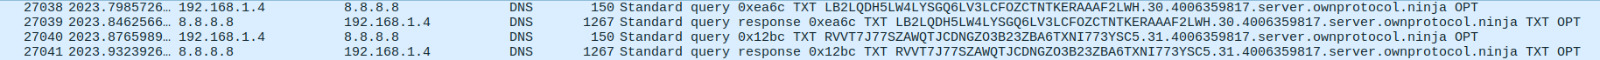
\includegraphics[width=0.9\textwidth]{ws_list.jpg}
    \caption{Captură Wireshark: Alternanța pachetelor}
    \label{fig:ws_list}
\end{figure}

\subsection{Analiza performanțelor și a rezilienței la rate limiting}
Rezultatele testelor de viteză, latență și pierdere de pachete sunt prezentate în Figura~\ref{fig:benchmarks}. Graficele au fost generate folosind biblioteca \textit{Matplotlib}~\cite{matplotlib}. Analiza metricilor arată impactul constrângerilor DNS asupra eficienței tunelului:

\begin{figure}[H]
    \centering
    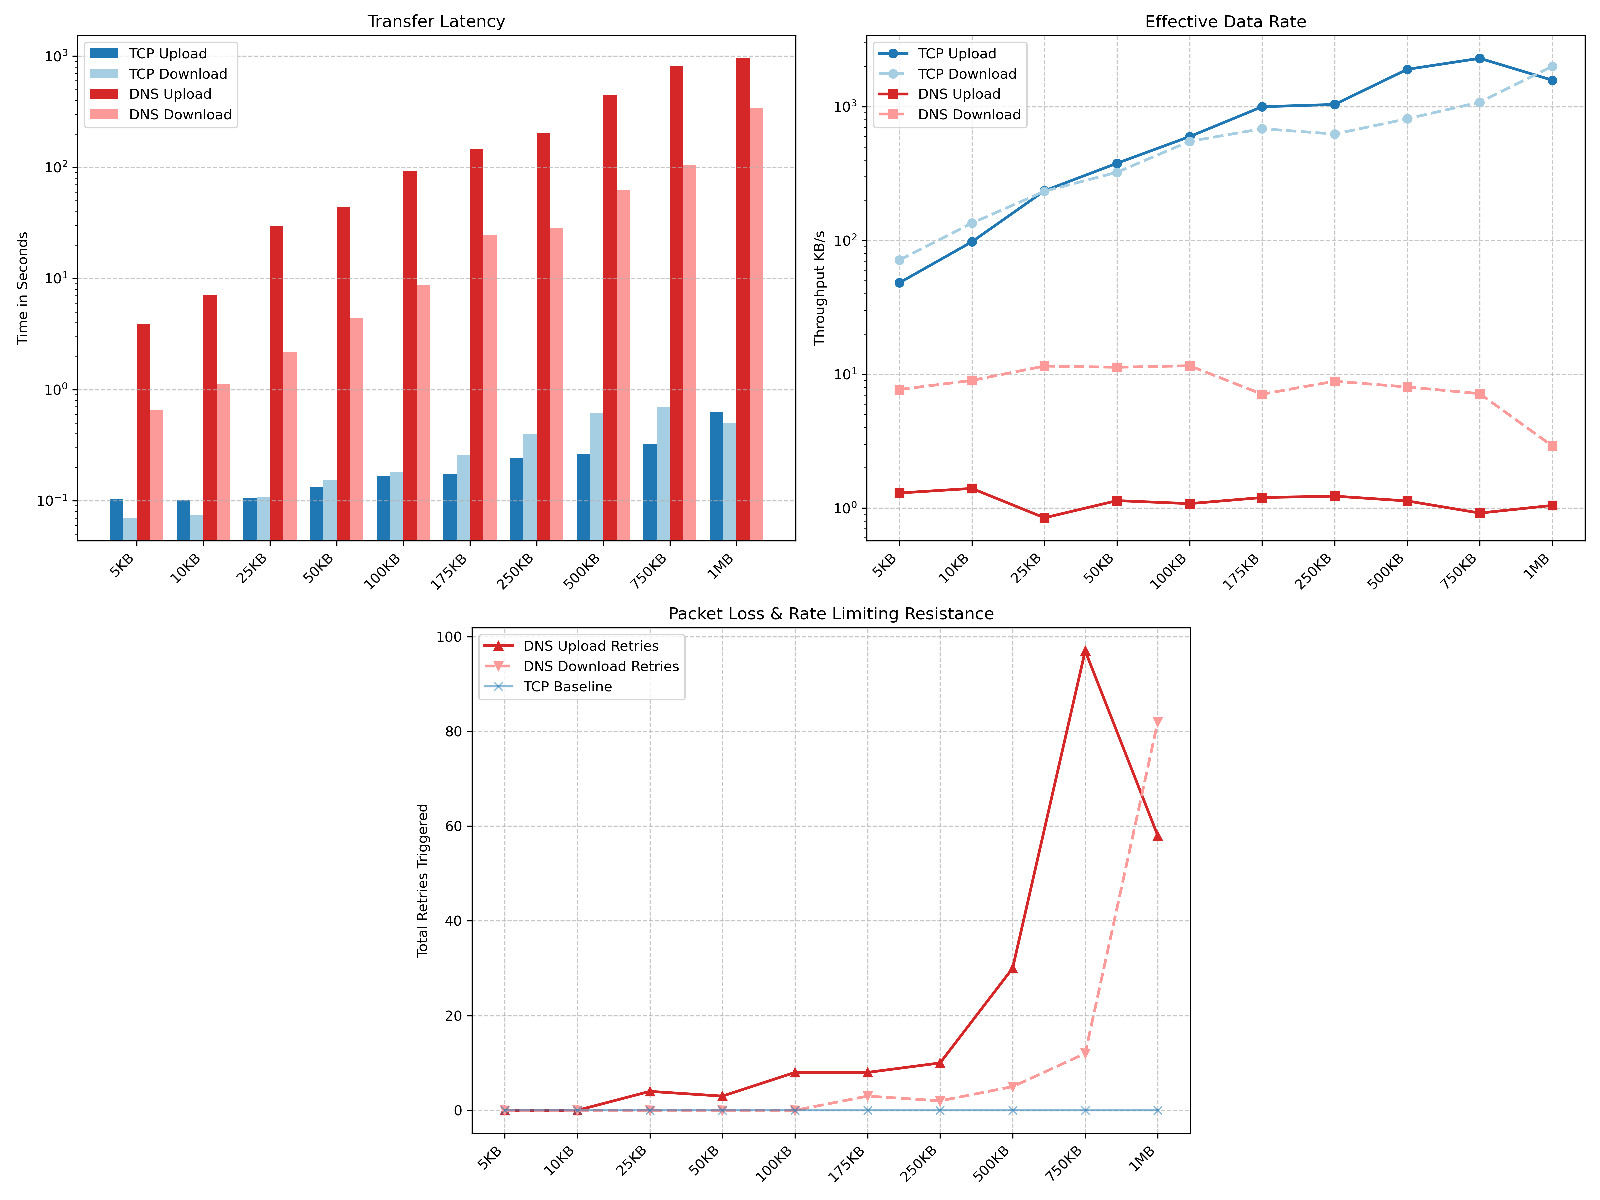
\includegraphics[width=\textwidth]{benchmark_results.jpg}
    \caption{Latența, lățimea de bandă și reziliența la Rate Limiting a protocolului}
    \label{fig:benchmarks}
\end{figure}

\begin{itemize}
    \item \textbf{Latența:} Asimetria dintre \textit{Upload} și \textit{Download} prin DNS este observabilă. Discrepanța validează ipoteza inițială: constrângerile de maxim 255 bytes per \texttt{QNAME} limitează viteza de \textit{Upload}, pe când utilizarea extensiei EDNS în \texttt{TXT} permite un \textit{Download} mai rapid. \textit{Baseline}-ul TCP se remarcă prin terminarea transferurilor extrem de rapid bidirecțional.
    
    \item \textbf{Lățimea de bandă:} Graficul al doilea evidențiază un eveniment clasic protocoalelor cu \textit{Sliding Window}: lățimea de bandă pentru TCP este proporțională dimensiunii fișierului, exemplificând \textit{TCP Slow Start}. În contrast, \textit{Throughput}-ul pentru tunelul DNS rămâne aproape constant. Comportamentul acesta relevă eficiența metodei \textit{Stop-and-Wait ARQ}, ce acționează ca un \textit{traffic shaper}, fără a trimite pachetele în \textit{burst}-uri.
    
    \item \textbf{Reziliența la Rate Limiting și Packet Loss:} Pentru fișierele de dimensiuni mici, de până la 250 KB, retransmisiile sunt minime, între 0 și 10 pachete. Începând cu pragul de 500 KB pierderile cresc alarmant, aproximativ 100 de retransmisii pentru \textit{Upload} la fișierul de 750 KB. Această zonă marchează activarea filtrelor de \textit{RRL}, ce încep să respingă cererile anormal de frecvente. Se observă că TCP-ul, protocol stabil ce nu suferă de \textit{rate limiting}, nu prezintă vreo pierdere de pachete.
\end{itemize}

Deși multe pachete sunt pierdute din cauza mecanismelor de protecție ale rețelei, bucla de retransmisie a păstrat conexiunea activă. Integritatea tuturor fișierelor reconstruite a fost validată criptografic prin SHA-256, rezultat ce demonstrează robustețea sistemului de control al fluxului implementat și a protocolului la \textit{rate limiting}.
\section{Concluzii}

\subsection{Realizarea lucrării}
Lucrarea a avut ca scop proiectarea și implementarea unui protocol de transport personalizat fiabil peste infrastructura DNS. Arhitectura a fost construită strict pe baza înregistrărilor de tip \texttt{TXT} și a interogărilor \texttt{QNAME}, utilizând protocolul UDP, ce ocupă portul 53. Prin dezvoltarea unui mecanism de controlare al fluxului de tip \textit{Stop-and-Wait ARQ}, sistemul a rezolvat problema pierderii de pachete inerentă rețelelor instabile, fără stare a sesiunii, și a mitigat declanșarea excesivă a filtrelor de \textit{Rate Limiting}. De asemenea, canalul de comunicație a fost securizat printr-un proces de \textit{handshake} bazat pe ECDHE autentificat printr-un HMAC dependent de un PSK, urmat de criptarea autentificată AES-GCM a tuturor pachetelor în care sunt transmise date.

\subsection{Rezultate și aplicații practice}
Rezultatele obținute confirmă funcționalitatea protocolului în situații practice, demonstrând o reziliență ridicată în fața mecanismelor de apărare ale rețelei, chiar și în condiții de pierdere masivă de pachete. Deși viteza de transfer este foarte limitată, în special la transmiterea \textit{upstream}, din cauza constrângerilor dimensionale ale protocolului DNS, acceptarea acestui compromis a fost necesară pentru a asigura o conexiune stabilă pe tot parcursul comunicării.

În practică, un astfel de sistem poate fi folosit ca \textit{fallback} pentru a administra la distanță echipamente ce se află în medii foarte stricte cu comunicarea externă. În cazurile în care porturile folosite de obicei pentru management (precum SSH sau RDP) sunt blocate de \textit{Firewall}-uri avansate, infrastructura DNS rămâne de cele mai multe ori unica modalitate de comunicație deschisă. Protocolul creat ar permite astfel executarea mentenanței de urgență sau recuperarea datelor din sistemele izolate. 

\subsection{Direcții de dezvoltare ulterioară}
Deși obiectivele inițiale au fost îndeplinite de implementarea instrumentului, există mai multe căi prin care protocolul poate fi îmbunătățit ulterior:
\begin{itemize}
    \item \textbf{Diminuarea entropiei informaționale:} Pentru micșorarea riscului de detecție din partea mecanismelor de tip NGFW, se poate adăuga un algoritm de (\textit{padding}) bazat pe dicționare. Intercalarea datelor codificate în \texttt{Base32} împreună cu șiruri de caractere ce aparțin limbajului natural ar reduce scorul entropic al etichetelor din domeniile generate. În plus, dacă s-ar adăuga un proces de dinamizare a dimensiunilor cererilor și răspunsurilor DNS, pericolul reprezentat de instrumentele pentru analiză euristică și statistică ar fi estompat.
    \item \textbf{Optimizarea controlului de flux:} Mecanismul strict de \textit{Stop-and-Wait}, bazat pe o buclă cu maxim 6 încercări și un \textit{timeout} de 3s pentru fiecare retransmisie, poate fi înlocuit cu o abordare mai flexibilă, fondată pe \textit{Leaky Bucket}. Această opțiune ar permite modificarea dinamică a ratei de transmisie, perfecționând lățimea de bandă, mai ales la \textit{download}, fără a trece pragurile de detecție ale filtrelor RRL.
    \item \textbf{Rotația domeniilor (\textit{Domain Flipping}):} Obținerea mai multor domenii autoritative (inclusiv a name serverelor aferente) și alternarea lor în timpul sesiunilor de tunelare. Această funcționalitate poate contribui la prevenția blocării fluxului de transfer al protocolului prin adăugarea unui singur domeniu pe un \textit{blacklist}.
\end{itemize}

\clearpage
\addtocontents{toc}{\setlength{\cftsecnumwidth}{2.2cm}}
\setcounter{section}{0}
\renewcommand{\thesection}{Anexa \arabic{section}}
\renewcommand{\theHsection}{anexa.\arabic{section}} %
\setcounter{figure}{0}
\setcounter{table}{0}
\renewcommand{\thefigure}{A\arabic{section}.\arabic{figure}}
\renewcommand{\thetable}{A\arabic{section}.\arabic{table}}
\section{Parametrii curbei eliptice SECP256R1}
\label{anexa:cripto_ec}
Securitatea algoritmului ECDHE se bazează pe dificultatea calculării logaritmului discret pe o curbă eliptică peste $\mathbb{Z}_p$ definită de ecuația $y^2 = x^3 + ax + b$ mod $p$, unde $4a^3 + 27b^2 \neq 0$ mod $p$. Constantele criptografice utilizate de protocol pentru curba \texttt{SECP256R1} sunt extrase din NIST SP 800-186~\cite{nist_sp800_186} și sunt enumerate în Tabela~\ref{tab:ec_specs}.

\begin{table}[htbp]
    \centering
    \small
    \renewcommand{\arraystretch}{1.1}
    \begin{tabular}{|c|>{\raggedright\arraybackslash}p{13cm}|}
        \hline
        \textbf{Parametru} & \textbf{Valoare Hexazecimal} \\
        \hline
        Ordinul prim $p$ & \texttt{FFFFFFFF00000001000000000000000000000000FFFFFFFFFFFFFFFFFFFFFFFF} \\
        \hline
        Coeficientul $a$ & \texttt{FFFFFFFF00000001000000000000000000000000FFFFFFFFFFFFFFFFFFFFFFFC} \\
        \hline
        Coeficientul $b$ & \texttt{5AC635D8AA3A93E7B3EBBD55769886BC651D06B0CC53B0F63BCE3C3E27D2604B} \\
        \hline
        Punctul de bază $G_x$ & \texttt{6B17D1F2E12C4247F8BCE6E563A440F277037D812DEB33A0F4A13945D898C296} \\
        \hline
        Punctul de bază $G_y$ & \texttt{4FE342E2FE1A7F9B8EE7EB4A7C0F9E162BCE33576B315ECECBB6406837BF51F5} \\
        \hline
        Ordinul $n$ & \texttt{FFFFFFFF00000000FFFFFFFFFFFFFFFFBCE6FAADA7179E84F3B9CAC2FC632551} \\
        \hline
    \end{tabular}
    \caption{Specificațiile curbei eliptice NIST P-256}
    \label{tab:ec_specs}
\end{table}

\section{Arhitectura operațională AES-GCM}
\label{anexa:cripto_aes-gcm}
Pentru criptarea autentificată protocolul folosește \textit{AES} în modul \textit{GCM}. Procesul este împărțit în fluxul de criptare/decriptare, pe baza funcției GCTR, și calcularea etichetei de autentificare prin funcția GHASH. Operațiile acestea sunt prezentate vizual în Figurile~\ref{fig:aes_enc}--\ref{fig:aes_ghash}, urmate de definițiile matematice, informațiile fiind preluate din \textit{NIST Special Publication 800-38D} ~\cite{nist_aesgcm}.

\begin{figure}[htbp]
    \centering
    \begin{minipage}[t]{0.48\textwidth}
        \centering
        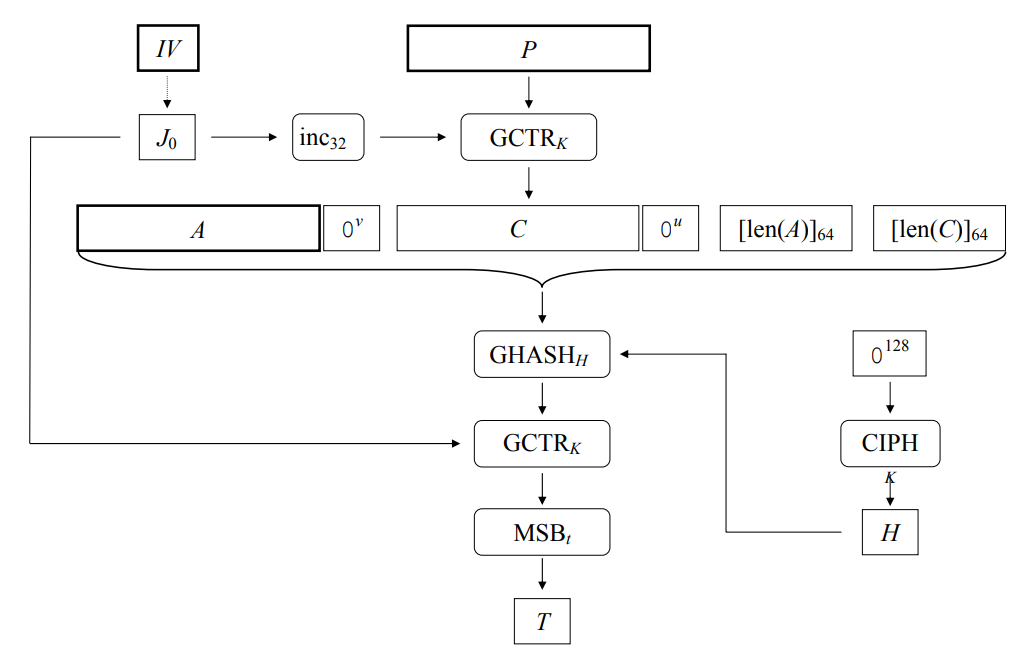
\includegraphics[width=\textwidth]{aes-gcm_encryption.png}
        \caption{Criptare AES-GCM}
        \label{fig:aes_enc}
    \end{minipage}\hfill
    \begin{minipage}[t]{0.48\textwidth}
        \centering
        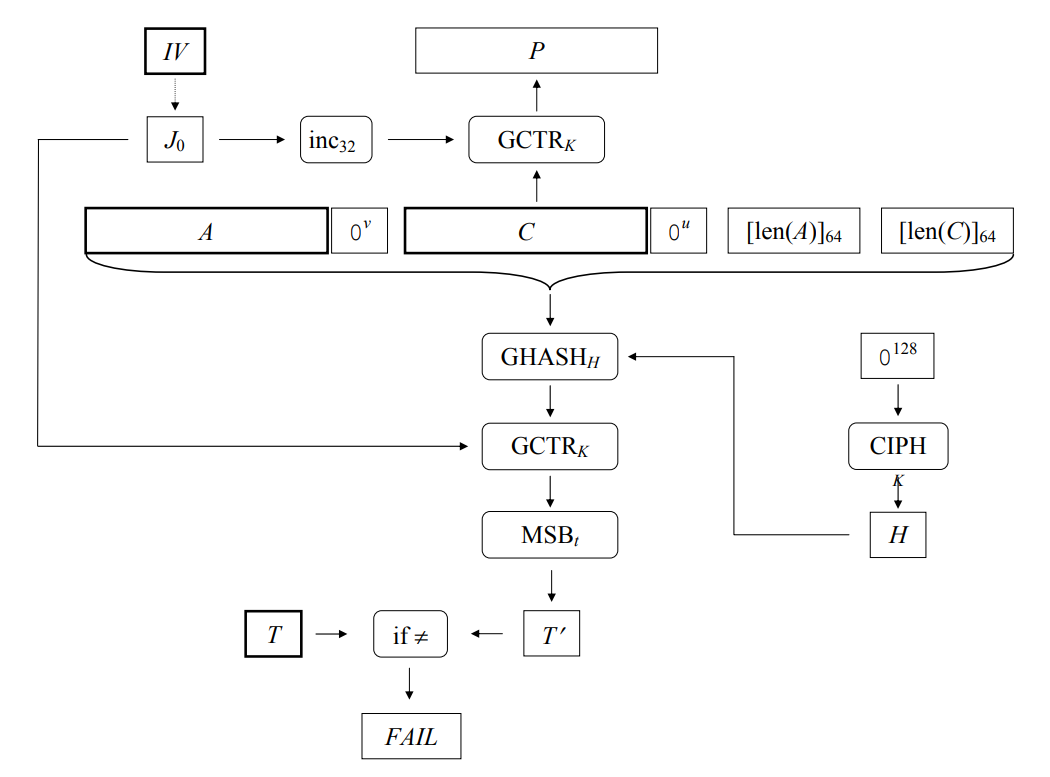
\includegraphics[width=\textwidth]{aes-gcm_decryption.png}
        \caption{Decriptare AES-GCM}
        \label{fig:aes_dec}
    \end{minipage}
\end{figure}

\vspace{0.2cm}

\begin{figure}[htbp]
    \centering
    \begin{minipage}[t]{0.48\textwidth}
        \centering
        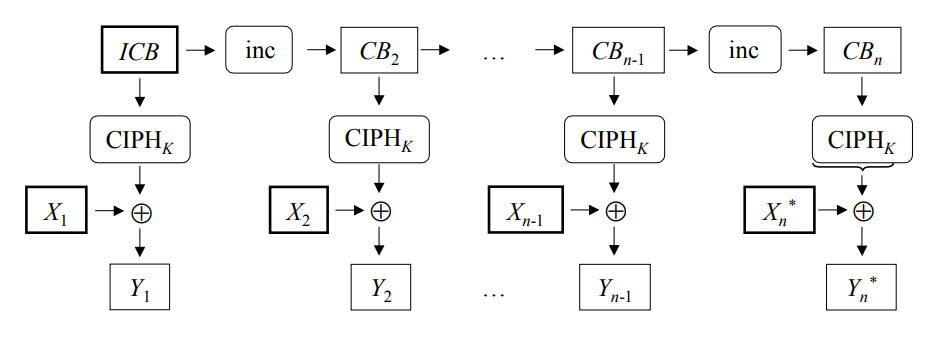
\includegraphics[width=\textwidth]{gctr_function.png}
        \caption{Operația GCTR}
        \label{fig:aes_gctr}
    \end{minipage}\hfill
    \begin{minipage}[t]{0.48\textwidth}
        \centering
        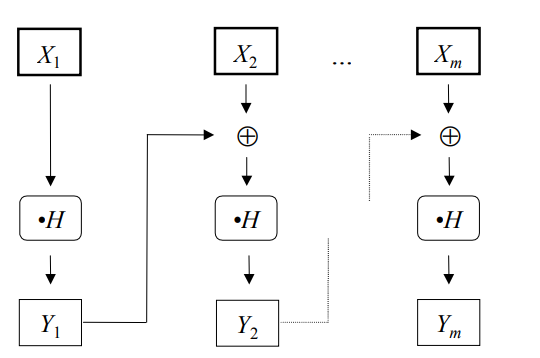
\includegraphics[width=\textwidth]{ghash.png}
        \caption{Generarea etichetei GHASH}
        \label{fig:aes_ghash}
    \end{minipage}
\end{figure}

\vspace{0.5cm}

\paragraph{Funcția GHASH}
Eticheta este calculată prin operații pe corpul finit Galois $\text{GF}(2^{128})$. Fie un șir de blocuri de 128 de biți $X_1, X_2, \dots, X_m$ și subcheia de hash $H = E_K(0^{128})$, funcția se definește iterativ:
$$ Y_i = (Y_{i-1} \oplus X_i) \cdot H $$
unde $Y_0 = 0^{128}$, și rezultatul $Y_m = \text{GHASH}_H(X)$. Înmulțirea se realizează modulo polinomul ireductibil $P(x) = x^{128} + x^7 + x^2 + x + 1$.

\paragraph{Funcția GCTR}
Criptarea este realizată prin modul \textit{CTR}. Pentru fiecare bloc de text în clar $X_i$ și valoarea contorului $CB_i$, textul cifrat $Y_i$ se calculează:
$$ Y_i = X_i \oplus E_K(CB_i) $$
unde $E_K$ este aplicarea algoritmului AES cu secretul $K$.

\paragraph{Criptarea autentificată}
Pentru a proteja atât datele adiționale ($A$), cât și textul cifrat ($C$), eticheta de autentificare finală $T$ (de lungime $t$) este calculată prin aplicarea funcției GHASH asupra concatenării acestora, urmată de o mascare XOR cu valoarea inițială a contorului criptat ($J_0$):
$$ T = \text{MSB}_t \left( \text{GHASH}_H(A \parallel 0^v \parallel C \parallel 0^u \parallel \text{len}(A)_{64} \parallel \text{len}(C)_{64}) \oplus E_K(J_0) \right) $$

\paragraph{Decriptarea autentificată}
La primire, procesul de decriptare verifică autenticitatea datelor înainte de a returna textul în clar, pentru prevenția atacurilor de tip \textit{chosen-ciphertext}. Eticheta anticipată $T'$ este recalculată, utilizând datele adiționale $A$ și textul cifrat primit $C$:
$$ T' = \text{MSB}_t \left( \text{GHASH}_H(A \parallel 0^v \parallel C \parallel 0^u \parallel \text{len}(A)_{64} \parallel \text{len}(C)_{64}) \oplus E_K(J_0) \right) $$

Validarea integrității și extragerea textului în clar $P$ se fac în baza condiției:
$$ P = 
\begin{cases} 
\text{GCTR}_K(J_0, C), & \text{dacă } T = T' \\ 
\mathit{FAIL}, & \text{dacă } T \neq T' 
\end{cases} 
$$

Dacă verificarea eșuează, se întoarce o eroare, iar blocurile decriptate sunt distruse din memorie, garantându-se că pachetele malformate pe rețea sunt respinse imediat.
\section{Analiza detaliată a pachetelor în Wireshark}
\label{anexa:wireshark}
Această anexă conține capturile de ecran realizate în timpul testărilor. 

\begin{figure}[H]
    \centering
    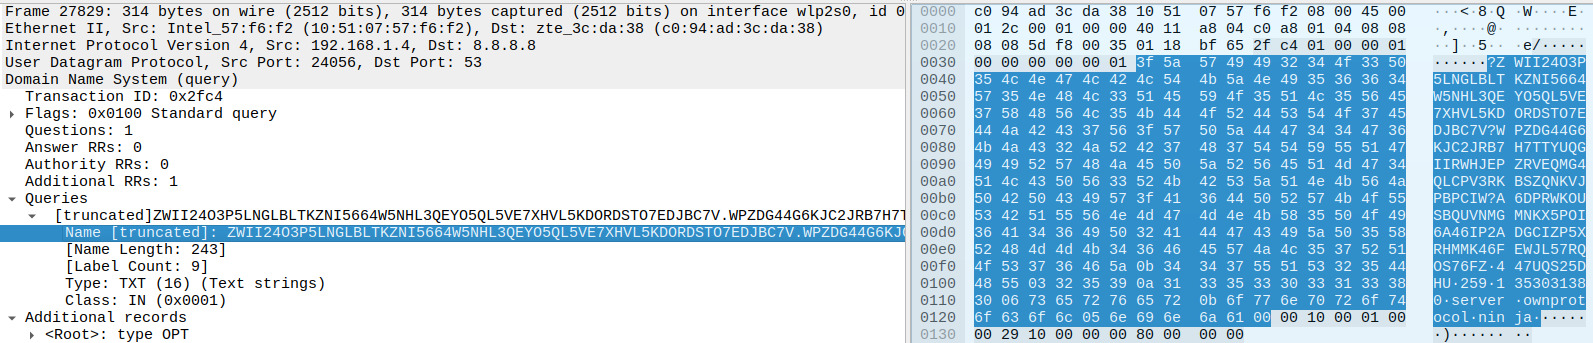
\includegraphics[width=0.9\textwidth]{ws_query.jpg}
    \caption{Detalierea QNAME-ului în traficul upstream}
    \label{fig:ws_detaliu_query}
\end{figure}

Conform analizei din Capitolul 4, Figura~\ref{fig:ws_detaliu_query} accentuează dimensiunea numelui de domeniu folosit în transferul de date. Similar, răspunsurile de la server prezintă structura conturată în Figura~\ref{fig:ws_detaliu_response}.

\begin{figure}[H]
    \centering
    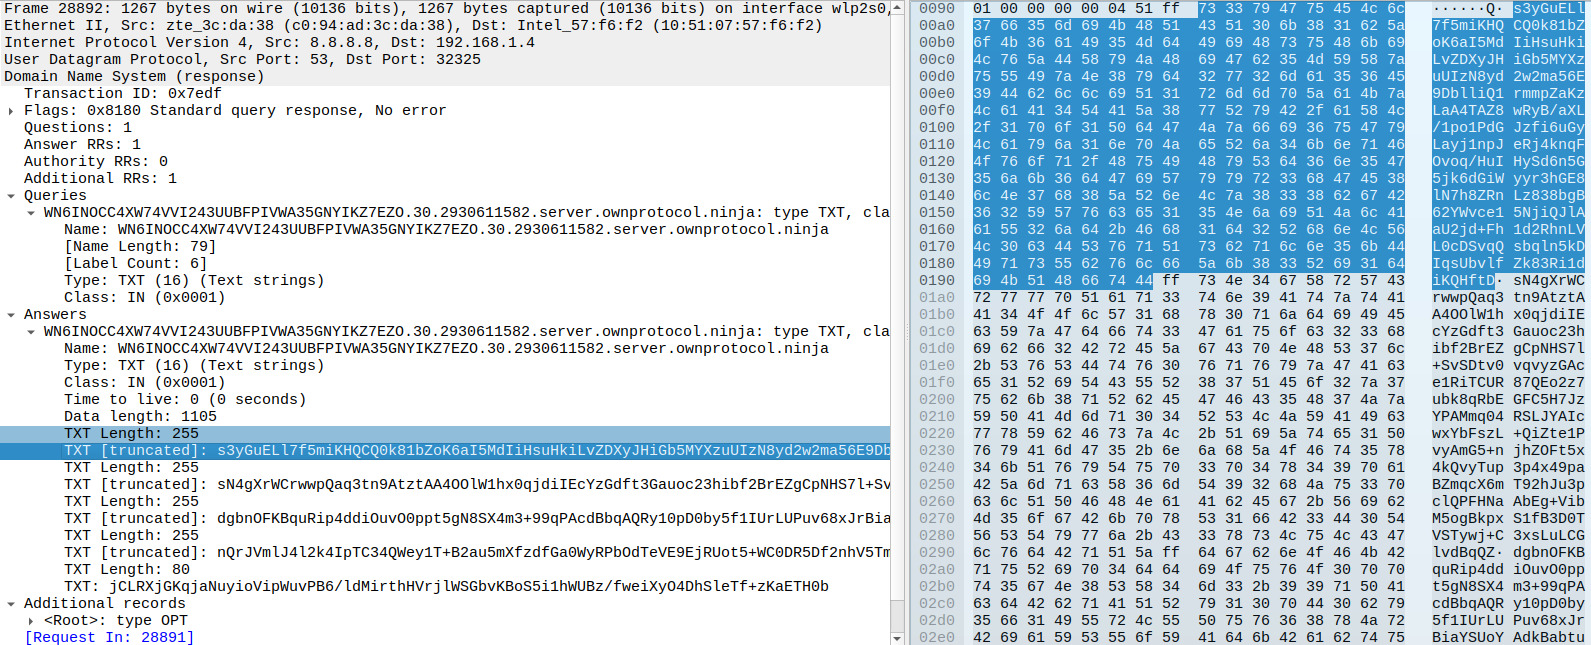
\includegraphics[width=0.9\textwidth]{ws_response.jpg}
    \caption{Detalierea răspunsului din downstream și a extensiei EDNS}
    \label{fig:ws_detaliu_response}
\end{figure}

\clearpage
\printbibliography[heading=bibintoc]

\end{document}